\documentclass[a4paper,12pt]{article}
\usepackage[utf8]{inputenc}
\usepackage[T1]{fontenc}
\usepackage[margin=2cm]{geometry}
\usepackage{fancyhdr}
\usepackage{lmodern}
\usepackage{graphicx}

\pagestyle{fancy}
\fancyhf{}
\fancyhead[L]{Technická dokumentácia}
\fancyhead[R]{Architektúra}
\fancyfoot[C]{\thepage}
\renewcommand{\headrulewidth}{0.4pt}
\renewcommand{\footrulewidth}{0pt}

\begin{document}

\begin{center}
  {\LARGE \textbf{Architektúra}} \\
  \vspace{1em}
  {\large Technická dokumentácia} \\
\end{center}

\section*{Úvod}

Tento dokument slúži ako časť technickej dokumentácie pre projekt Zdieľané supervízne riadenie dronov vo virtuálnej realite. 

Obsahuje popis architektúry systému, využité technológie a použité topiky v rámci ROS2. 

Je určený pre vývojárov, ktorý budú vyvýjať a rozvýjať systému. 

Neobsahuje detailné informácie o implementácii jednotlivých komponentov, ale poskytuje prehľad o štruktúre a komponentoch systému.


\newpage\renewcommand{\contentsname}{Obsah}\tableofcontents


\newpage

\section{Architektúra systému}

Vyzuálne architektúra systému je znázornená na obrázku \ref{fig:architektura}:

\begin{figure}[h!]
\centering
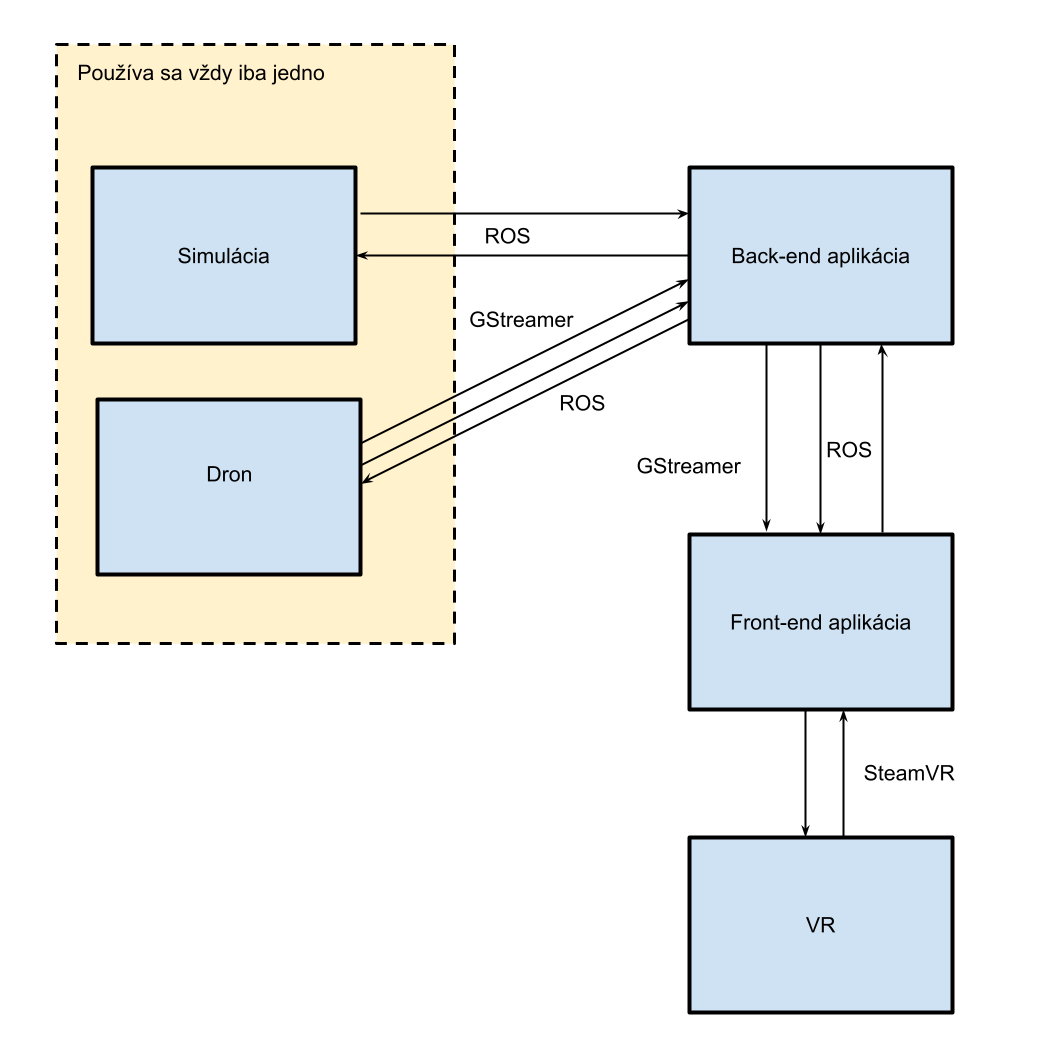
\includegraphics[width=0.8\textwidth]{img/arch.png}
\caption{Architektúra systému}
\label{fig:architektura}
\end{figure}

Systém sa skladáz z 2 aplikácií, ktoré zabezpečujú obojsmernú komunikáciu medzi dronmi a virtuálnou realitou.

Prvou je backendová aplikácia bežica na ROS2, ktorá zabezpečuje kominikáciu s dronmi a automatické riadenie dronov 
po predefinovaných trajektóriach. Takiež zabezpečuje bezpečnosť pri riadené dronov, vyhnutie sa kolíziám a konverziu
videa z simulácie do GStreameru, ktorý následne posiela video do frontendovej aplikácie.

Frontendová aplikácia využíva sa pripája na backendovú aplikáciu pomocou ROS2 bridge a GStreameru
a zabezpečuje zobrazenie dronov a možnosť ovládania dronov. Na zobrazenie vo virtuálnej realite používa
SteamVR a OpenVR, ktoré zabezpečujú prenos kontentu z obrazovky počítača do VR headsetu a umožnujú spracovať 
používateľské vstupy z VR ovládačov.

\newpage
\section{Komunikácia medzi komponentami}

\subsection{Dron a backendová aplikácia}

Drony komunikujú s backendovou aplikáciou pomocou ROS topikov/servisov a v prípade reálneho drono zdieľanie videa prebieha pomocou GStreameru.

\subsubsection*{Backend sa pripája na topiky:}

\begin{itemize}
    \item \textbf{/dronX/stop} - std\_msgs/msg/Bool - požiadavka na zastavenie misie a pristátie po dokončení aktuálneho cyklu
    \item \textbf{/dronX/mavros/state} - mavros\_msgs/msg/State - aktuálny stav dronu (stav pripojenia, mód letu, armed stav)
    \item \textbf{/dronX/mavros/local\_position/pose} - geometry\_msgs/msg/PoseStamped - aktuálna lokálna pozícia dronu
\end{itemize}

\subsubsection*{Ďalej publikuje topiky, na ktoré sa dron pripája:}

\begin{itemize}
    \item \textbf{/dronX/mavros/setpoint\_position/local} - geometry\_msgs/msg/PoseStamped - publikovanie cieľovej pozície počas navigácie medzi waypointmi
\end{itemize}

\subsubsection*{A na ovládanie drona využíva servisy:}

\begin{itemize}
    \item \textbf{/dronX/mavros/set\_mode} - mavros\_msgs/srv/SetMode - prepnutie letového režimu dronu (napr. GUIDED)
    \item \textbf{/dronX/mavros/cmd/arming} - mavros\_msgs/srv/CommandBool - arm/disarm dronu
    \item \textbf{/dronX/mavros/cmd/takeoff} - mavros\_msgs/srv/CommandTOL - vzlet dronu do zadanej výšky
    \item \textbf{/dronX/mavros/cmd/land} - mavros\_msgs/srv/CommandTOL - pristátie dronu
\end{itemize}


\subsection{Backendová a frontendová aplikácia}

Backendová a frontendová aplikácia spolu komunikujú cez rozhranie ROS2 bridge, 
ktoré umožňuje prenos správ a dát medzi ROS2 aplikáciami a aplikáciami nevyužívajúcimi ROS2.
Tento spôsob sme zvolili z dôvodu vyššej portability aplikácie, bez nutnosti implementovať ROS2 klienta priamo vo VR aplikácii.

\subsubsection*{Front end sa prípája na topiky (pre každý dron zlášť):}

\begin{itemize}
    \item \textbf{/dronX/local\_position/pose} - geometry\_msgs/msg/PoseStamped - aktuálna pozícia robota
    \item \textbf{/dronX/battery} - sensor\_msgs/msg/BatteryState - stav batérie robota
    \item \textbf{/dronX/state} - mavros\_msgs/msg/State - aktuálny stav robota/dronu
    \item \textbf{/dronX/setpoint\_velocity/cmd\_vel\_unstamped} - geometry\_msgs/msg/Twist - publikovanie rýchlostných príkazov
\end{itemize}

\subsubsection*{Front end na ovládanie robota využíva servisy:} 

\begin{itemize}
    \item \textbf{/supervisor/takeover\_request} - std\_msgs/msg/String - prevzatie kontroly
    \item \textbf{/supervisor/release\_request} - std\_msgs/msg/String - skončenie manuálneho režimu
    \item \textbf{/supervisor/manual\_cmd\_vel} - geometry\_msgs/msg/Twist - ovládanie smeru robota
\end{itemize}

Video je stremované pomocou GStreamer-u. 

\subsection{Frontendová aplikácia a VR headset}

Frontendová aplikácia využíva SteamVR a OpenVR na komunikáciu s VR headsetom, ktoré zabezpečuje prenos obrazu z počítača
a spätné čítanie vstupov z VR ovládačov, ktoré vieme následne v aplikácii spracovať a ovládať tak drona. 

\end{document}
